\documentclass[]{article}
\usepackage{lmodern}
\usepackage{amssymb,amsmath}
\usepackage{ifxetex,ifluatex}
\usepackage{fixltx2e} % provides \textsubscript
\ifnum 0\ifxetex 1\fi\ifluatex 1\fi=0 % if pdftex
  \usepackage[T1]{fontenc}
  \usepackage[utf8]{inputenc}
\else % if luatex or xelatex
  \ifxetex
    \usepackage{mathspec}
  \else
    \usepackage{fontspec}
  \fi
  \defaultfontfeatures{Ligatures=TeX,Scale=MatchLowercase}
\fi
% use upquote if available, for straight quotes in verbatim environments
\IfFileExists{upquote.sty}{\usepackage{upquote}}{}
% use microtype if available
\IfFileExists{microtype.sty}{%
\usepackage[]{microtype}
\UseMicrotypeSet[protrusion]{basicmath} % disable protrusion for tt fonts
}{}
\PassOptionsToPackage{hyphens}{url} % url is loaded by hyperref
\usepackage[unicode=true]{hyperref}
\hypersetup{
            pdftitle={MARCO TEÓRICO},
            pdfauthor={Casallas - Espinel - Rodríguez},
            pdfborder={0 0 0},
            breaklinks=true}
\urlstyle{same}  % don't use monospace font for urls
\usepackage{graphicx,grffile}
\makeatletter
\def\maxwidth{\ifdim\Gin@nat@width>\linewidth\linewidth\else\Gin@nat@width\fi}
\def\maxheight{\ifdim\Gin@nat@height>\textheight\textheight\else\Gin@nat@height\fi}
\makeatother
% Scale images if necessary, so that they will not overflow the page
% margins by default, and it is still possible to overwrite the defaults
% using explicit options in \includegraphics[width, height, ...]{}
\setkeys{Gin}{width=\maxwidth,height=\maxheight,keepaspectratio}
\IfFileExists{parskip.sty}{%
\usepackage{parskip}
}{% else
\setlength{\parindent}{0pt}
\setlength{\parskip}{6pt plus 2pt minus 1pt}
}
\setlength{\emergencystretch}{3em}  % prevent overfull lines
\providecommand{\tightlist}{%
  \setlength{\itemsep}{0pt}\setlength{\parskip}{0pt}}
\setcounter{secnumdepth}{0}
% Redefines (sub)paragraphs to behave more like sections
\ifx\paragraph\undefined\else
\let\oldparagraph\paragraph
\renewcommand{\paragraph}[1]{\oldparagraph{#1}\mbox{}}
\fi
\ifx\subparagraph\undefined\else
\let\oldsubparagraph\subparagraph
\renewcommand{\subparagraph}[1]{\oldsubparagraph{#1}\mbox{}}
\fi

% set default figure placement to htbp
\makeatletter
\def\fps@figure{htbp}
\makeatother


\title{MARCO TEÓRICO}
\author{Casallas - Espinel - Rodríguez}
\date{}

\begin{document}
\maketitle

\section{Brecha Digital}\label{brecha-digital}

En el año 1995 eclosionan para la población dos tecnologías totalmente
disruptivas, el internet y la telefonía móvil, ellas sugieren una nueva
revolución, la llamada revolución digital, que a su vez crea la sociedad
de la información(S.I), dando inicio al planteamiento sobre cómo medir y
modelizar la S.I, el nivel de desarrollo digital y el impacto del
desarrollo digital en el ser humano.De igual manera, el acceso a
internet a través de las Tecnologías de la información y las
comunicaciones (TIC) ha tenido un auge exponencial en los últimos años,
en efecto, este avance se presenta en países desarrollados o zonas
metropolitanas de países en desarrollo {[}sen{]}, sin embargo, existen
unas comunidades con poco o ningún acceso a las TIC {[}maseratti{]} y
otras con acceso casi universal a telefonía fija, móvil e Internet de
banda ancha, es así que resulta el concepto de Brecha Digital
entendiendose como la ausencia de una o varias dimensiones contenidas en
el desarrollo digital. En relación con lo anterior, las poblaciones sin
acceso a las TIC poseen un bajo nivel socioeconómico, viven en zonas de
difícil acceso con condiciones climatológicas desfavorables e incluso
con ineficiencia o inexistencia de redes eléctricas, al mismo tiempo,
las personas que viven en áreas rurales sufren el efecto de la brecha
digital incluso más fuerte que los habitantes urbanos, debido a que no
pueden acceder a servicios como el aprendizaje a distancia, la salud y
el comercio electrónico {[}Bernardi{]}.

\section{Redes Libres}\label{redes-libres}

\section{Planeación de Redes
Inalámbricas}\label{planeaciuxf3n-de-redes-inaluxe1mbricas}

Con el objetivo de reducir la brecha digital, autores {[}Bernardi,
maseratti, sen{]} han propuesto como solución la planeación y despliegue
de redes de banda ancha inalámbrica en zonas rurales. Para ello es
necesario hablar de conectividad , siendo un factor clave que hace
alusión a la disponibilidad que tiene un dispositivo para conectarse a
otro o conectarse a una red, es por eso, que cerrar esta brecha requiere
proporcionar conectividad a internet en todos los pueblos.

La planeación de redes inalámbricas es un área muy activa por la
comunidad científica, sin embargo el foco de las investigaciones son las
redes de banda ancha móvil y las redes de área local inalámbrica.

\subsection{Factores clave}\label{factores-clave}

A continuación se detallan factores innatos claves de la planeación de
redes inalámbricas.

\begin{itemize}
\tightlist
\item
  Costos de depliegue:
\item
  Costos de implementación:
\item
  Expansión de la red: Creciemiento de la red, abarcando más territorio
\item
  Coberturad de la red: En zonas rurales prevalece mantener la cobertura
  de servicios de internet en diferentes lugares sobre la capacidad.
\item
  Capacidad de la red: Ancho de banda requerido para la transferencia de
  datos
\item
  Retorno de la inversión: Referente para pequeños proveedores de
  internet inalámbrico (WISP)
\item
  Sector económico y social de la población rural: Delimitantes
  socioeconómicos del poder adquisitivo de los habitantes
\end{itemize}

\section{Algoritmos utilizados en la
planeación}\label{algoritmos-utilizados-en-la-planeaciuxf3n}

Aunque existen estructuras de algoritmos para solucionar problemáticas
en la planeación incremental de redes inalámbricas {[}Whitaker{]}
también proporciona información acerca de los enfoques propuestos para
el diseño de redes, que muestran la evolución de modelos y técnicas para
la planificación automática de servicios inalámbricos celulares, cabe
resaltar que la documentación existente hace énfasis en redes móviles,
sin embargo, este concepto es aplicable para el despliegue de redes
inalámbricas rurales. Dicho lo anterior, whitaker facilita la
descripción de diferentes clases de algoritmos que se pueden usar para
realizar la planeación automática de redes inalambricas.

\begin{itemize}
\tightlist
\item
  \textbf{Algoritmos codiciosos} 
\end{itemize}

\begin{itemize}
\item
  Codiciosos (o secuenciales) los algoritmos simplemente ponen en marcha
  y configuran los transmisores de la mejor manera posible en algún
  orden, sin que sea posible la reconfiguración o la puesta en marcha.
  Estos enfoques se utilizan para generar una red inicial y tener un
  mayor desarrollo. Un problema crucial se relaciona con la forma en que
  se ordenan los sitios candidatos y las configuraciones antes de
  aplicar el algoritmo. Tales métodos, por ejemplo, han sido
  investigados por problemas relacionados con la gráfica y la asignación
  de frecuencia en {[}11, 12{]}.
\item
  \textbf{Algoritmos exactos} Existe una variedad de algoritmos que son
  capaces de buscar una solución exacta a un problema. Estos enfoques
  deben probar todas las combinaciones posibles de diseños de red
  potenciales y, con frecuencia, operar rechazando soluciones que
  contengan redes o redes parciales no deseables. Los algoritmos que
  operan sobre esta base incluyen el seguimiento y la verificación hacia
  adelante. Sin embargo, debido a la naturaleza difícil del problema,
  los algoritmos de este tipo solo pueden ejecutarse hasta el
  agotamiento en pequeños problemas de prueba. En consecuencia, se
  pueden relajar con una terminación temprana o usarse para explorar
  selectivamente regiones limitadas desde el espacio de búsqueda de
  todos los diseños de red posibles, como en {[}32, 33, 34, 44{]}.
\item
  \textbf{Algoritmos genéticos (GA)} Estos algoritmos imitan algunos de
  los procesos de evolución y selección natural al mantener una
  población de soluciones candidatas que están representadas por una
  cadena de genes (con frecuencia binarios). Con el tiempo, la población
  evoluciona a través de procesos que emulan procesos biológicos como la
  reproducción. Los miembros de la población se combinan para producir
  descendientes. Introducido por Holanda {[}21{]}, el concepto básico es
  que los fuertes tienden a adaptarse y sobrevivir, mientras que los
  débiles tienden a desaparecer. Los artículos {[}29, 28, 19, 22, 13{]}
  muestran enfoques para la planificación celular utilizando GA.
\item
  \textbf{Annealing Simulado (SA)} Annealing simulado (SA) es una
  meta-heurística derivada de la mecánica estadística. El método opera
  utilizando el principio de vecindad y mide soluciones potenciales
  usando una función de costo. Permite que la búsqueda continúe con la
  función de costo, lo que reduce la mayor parte del tiempo (suponiendo
  una minimización), pero la función de costo puede aumentar
  ocasionalmente para permitir el escape de mínimos locales que no son
  globales. Las posibilidades de aceptar una solución peor están
  controladas por un parámetro en el algoritmo. El procedimiento de
  recocido simulado de Kirkpatrick et al. {[}27{]} varía este parámetro
  utilizando un programa de recocido que generalmente reduce la
  posibilidad de escapar de los mínimos locales con el tiempo. Para un
  tratamiento detallado del recocido simulado, se hace referencia al
  lector {[}2{]}. Los enfoques para la planificación celular en {[}4,
  10, 31, 6, 23{]}
\item
  \textbf{Tabu Search (TS)} La técnica meta-heurística (TS) de búsqueda
  de tabúes opera utilizando el principio de vecindad como para escalar
  colinas. Sin embargo, en un intento por evitar los ciclos y
  proporcionar un mecanismo para escapar de soluciones óptimas pero no
  globales, algunos movimientos, en una iteración particular, pueden
  clasificarse como tabú o tabú. Los movimientos se clasifican como tabú
  al considerar el historial a corto y largo plazo de la secuencia de
  movimientos. También hay criterios de aspiración que anulan los
  movimientos de tabú si se aplican circunstancias particulares.
\item
  \textbf{Algoritmos de adaptación para diseño de red automático} El
  diseño automático de la red se puede realizar para poner en marcha los
  transmisores de varias maneras. El software puede estar diseñado para
  comisionar un número exacto o un número máximo fijo de transmisores, o
  puede tener total libertad. Estos objetivos pueden afectar
  significativamente la forma en que se aborda el problema y se diseña
  el algoritmo. Adicionalmente la aplicación de algoritmos debe tener en
  cuenta resolver conflictos y tensiones. Con respecto a la puesta en
  marcha de los transmisores, los transmisores de alta potencia y poco
  distribuidos pueden proporcionar una cobertura adecuada al tiempo que
  minimizan los costos pero puede proporcionar una capacidad de red
  inadecuada. Además, las regiones de entrega pueden ser difíciles de
  establecer sin instanciar las regiones de interferencia en este
  escenario. Definir los objetivos operativos deseados debe ser
  considerado. El gasto computacional y de infraestructura para
  proporcionar el último porcentaje de la cobertura máxima posible o la
  utilización del tráfico puede ser significativo. A nivel de
  configuración de infraestructura, la inclinación, el acimut, la
  configuración de potencia máxima y la elección de la antena y la
  sectorización están disponibles para sintonizar en sitios comisionados
  si el algoritmo no se limita a elegir transmisores preconfigurados. Es
  importante destacar que estos parámetros son cruciales para el
  dimensionamiento de la celda, es decir, un ajuste fino para
  proporcionar un traspaso y una interferencia máxima adecuada. Tenga en
  cuenta que estos objetivos pueden ser difíciles de satisfacer si solo
  se especifican instancias limitadas de preconfiguración en los sitios
  potenciales.
\end{itemize}

\section*{ESTADO DEL ARTE}\label{estado-del-arte}
\addcontentsline{toc}{section}{ESTADO DEL ARTE}

\section{Redes móviles UMTS}\label{redes-muxf3viles-umts}

De igual forma en {[}Hitlarie2008{]}, se presenta una literatura
detallada de los problemas que se presentan en la planeación de la
topología celular 3G, la cual, esta basada en el Sistema universal de
telecomunicaciones móviles \textbf{UMTS} (``\emph{Universal Mobile
Telecommunications System}''); para entender las dificultades que se
presentan en la planeación, es importante hacer una pequeña descripción
de la arquitectura UMTS.

Una arquitectura típica de UMTS se muestra en la figura (1), donde se
observa que una red UMTS esta dividida en dos partes: la \emph{red de
acceso} y la \emph{red de núcleo}. La primera, es también llamada red
UMTS de radio terrestre \textbf{UTRAN}, la cual esta compuesta por
muchos subsistemas de red de radio \textbf{RNS} (``\emph{radio network
subsystem}''). Cada RNS contiene un controlador de red de radio
\textbf{RNC} (``\emph{radio network controller}'' ) y una o mas
estaciones bases \emph{BS} (``\emph{base estation}'').

Las estaciones bases (en este caso son los \emph{nodos B}) son usados
para trasmitir/recibir radiofrecuencia hacia/desde los usuarios móviles,
mientras que las RNC se ocupa de los recursos y la gestión de trafico de
datos. El principal objetivo de la UTRAN (``\emph{UMTS Terrestrial Radio
Access Network}'') es hacer el enlace entre los usuarios móviles y el
núcleo red.

\subsection{Planeación de Celda}\label{planeaciuxf3n-de-celda}

El autor \emph{Hitlarie}, descompone la planeación de las redes móviles
de manera modular, con el fin de reducir la complejidad y los divide en
los siguientes subproblemas:

\begin{itemize}
\tightlist
\item
  Subproblemas de planeación de celdas.
\item
  Subproblemas de planeación de red de acceso.
\item
  Subproblemas de planeación de núcleo de red.
\end{itemize}

La parte de los subproblemas que se necesita abordar con más detalle,
son los de planeación de celdas, ya que se asemeja más al enfoque que se
necesita en la planeación de redes inalámbricas de banda ancha; a
continuación se describe dicho subproblema, así como algunos trabajos
que se han realizado.

\textless{}-- Descripción \ldots{} --\textgreater{} \#\#\# Subproblema
de celdas o localización de estación base

El problema inicial de planeación es cubrir todos los usuarios móviles
en un determinado área con el número mínimo de BSs. En la planeación de
celdas se encarga de resolver los siguientes items:

\begin{itemize}
\tightlist
\item
  Optimizar el número de BSs.
\item
  Mejor localización para instalar BSs.
\item
  Escoger el tipo o modelo de BSs.
\item
  Configuración (altura, orientación, potencia, etc).
\item
  Asignación de usuarios móviles a la BS.
\end{itemize}

Los problemas de planeación pueden variar dependiendo en la planeación
de red objetivo. Usualmente, en la planeación de red se requiere
minimizar los costos de la red, maximizar la calidad de la señal y
maximizar el área de cobertura. Sin embargo esto puede ser
contradictorio,ya que por ejemplo, si se quiere maximizar la cobertura
se necesitaran desplegar mas BSs y esto por supuesto, aumentara los
costos.

Al principio la planeación de redes inalámbricas se realizaba teniendo
en cuenta la predicción de la señal, sin embargo en las redes UMTS, la
planeación de radio no puede ser solo basado en la predicción de la
señal sino que se deben tener en cuenta la distribución de trafico. En
esta parte aparece gran cantidad de literatura del autor Amaldi,en
\cite{Amaldi2003}, el autor contextualiza que en la planeación de radio
en el El sistema global para las comunicaciones móviles \textbf{GSM}
(``Global System for Mobile communications'') se realizaba en dos fases,
la fase de planeación de cobertura donde se define la mejor localización
de las BSs teniendo en cuenta los modelos de propagación y la fase de
planeación de frecuencia, que define el numero de canales para cada BS
teniendo en cuenta la calidad de la señal de interferencia de radio
\textbf{SIR} (``Signal-to-Interference Ratio'').

Sin embargo, teniendo en cuenta el Acceso múltiple por división de
código de banda ancha W-CDMA(``Wideband Code Division Multiple
Access''), esto ya no se puede realizar en estas dos fases, debido a que
el ancho de banda es compartido por todas las conexiones activas y no
por la frecuencia asignada, así como también el área de cobertura de
cada BS es afectada por la cantidad de trafico.

Para la planeación de celdas, se tiene en cuenta los parámetros de
calidad de la SIR, en el cual se define una SIR mínima, el cual depende
de la potencia recibida; Esta depende de la potencia trasmitida y las
atenuaciones de señal en la propagación, por ende la potencia trasmitida
se puede ajustar para minimizar la interferencia, aquí aparece un
concepto importante, el cual es el control de potencia
\textbf{PC}(``\emph{power control}''), en donde se ajusta la potencia de
trasmisión para cumplir dos objetivos, la potencia objetivo recibida
\(P_{tar}\) y la SIR objetivo \(SIR_{tar}\). En este articulo
\emph{Amaldi} propone un modelo de programación matemática, que ayuda en
la decisión de planear redes móviles, teniendo en cuenta la mejor
localización y configuración de las BSs, teniendo en cuenta el modelo de
propagación \emph{Hata}, donde se ajusta el PC y este a su vez es
probado con un algoritmo aleatorio voraz, el cual añade o remueve BSs de
la topología; En este artículo se describe el rendimiento de esta
solución dando resultados óptimos y también demuestra que este problema
es un problema típico de NP-hard.

En la planeación de redes, ha menudo se utiliza la optimización de
varios objetivos, mas conocido como optimización multi-objetivo, el cual
es diferente de una optimización simple , puesto que aquí solo importa
optimizar un parámetro, dando como resultado el mejor diseño o la mejor
optimización, teniendo en cuenta un máximo o un mínimo global que
dependerá del objetivo de la optimización (maximizar o minimizar), sin
embargo en la optimización multi-objetivo, existe mas de una solución
optima con respecto a todos los objetivos; aquí, el objetivo consiste en
encontrar un optimo de pareto, el cual nos dice que una solución es
optima cuando no existe otra solución tal que mejore en un objetivo sin
empeorar al menos uno de los otros.

Como se ha visto anteriormente, en la planeación se pueden abordar
diferentes objetivos(lugar de instalación de BS, configuración, altura,
potencia, etc), sin embargo, al momento de planificar la red, atacar
todos los problemas al tiempo es un problema complejo, por esto, se han
venido implementando algoritmos multi-objetivos, generalmente para estos
casos se han venido desarrollando algoritmos genéticos AG, en el trabajo
de (Raisanen and Whitaker, 2005), los autores recolectan cuatro estados
del arte de algoritmos genéticos multi-objetivo, donde los ponen a
prueba para planificar una red aumentando la cobertura teniendo en
cuenta los costos y los comparan teniendo en cuenta su desempeño en
ciertas pruebas sintetizadas ; los autores toman como referencia los
algoritmos: \textbf{SPEA2}, \textbf{NSGAII}, \textbf{PGSA} y
\textbf{SEAMO}. A continuación de hará una breve descripción de cada
uno.

\begin{itemize}
\tightlist
\item
  \textbf{SPEA2} (\emph{The Strength Pareto Evolutionary Algorithm
  version II}):
\end{itemize}

La población inicial es sometida a un fittness (aptitud), donde se
escoge el valor individual mas \emph{fit} de la unión del archivo y la
población hija. El valor de fitness, esta dado por la suma de dos
partes, \emph{raw fitness}, el cual esta dada por cuantas soluciones
domina y la \emph{densidad estimada}, el cual es la proximidad de otras
soluciones en el espacio objetivo. Cada generación \(n\) es guardada en
el archivo, en donde es de nuevo aplicado el operador a la nueva
generación; Este proceso se repite hasta terminar el proceso.

\begin{itemize}
\item
  \textbf{NSGA II} El individuo mas \emph{fit} esta determinado por la
  unión del archivo y la población hijo, determinado por mecanismos de
  clasificación compuesto de dos partes. La primera parte esta compuesta
  al determinar la capa de soluciones que no son dominadas, es decir,
  las que están mas cerca al frente de pareto. La segunda parte es una
  medida de dispersión, determinada por la distancia de hacinamiento
  crowding distance), el cual se escogerá el que tenga menor
  hacinamiento, puesto que esto significa que tendra mas población
  cubierta y la solución sera mas diversificada. Este proceso se
  repetira \(n\) repeticiones, guardando el valor de los dos resultados
  y repitiendo lo mismo con las nuevas generaciones, hasta que el
  algoritmo finalice.
\item
  \textbf{PESA} (\emph{The Pareto Envelope-based Selection Algorithm})
\end{itemize}

A diferencia de los dos algoritmos anteriores, el \emph{PESA} no tiene
un tamaño de archivo fijo y solo permite que las soluciones no dominadas
sean miembros, por ende es mas limitado. Si el archivo excede el tamaño
de \(n\) soluciones, un factor \emph{squeeze} o factor de compresión, es
calculado para todos los miembros del archivo. El factor de
\emph{squeeze} es el total de miembros en una subregión en una
cuadricula (las que están en el espacio de búsqueda, dentro de la
subregión). El factor \emph{squeeze} mas alto es el que tenga mas
vecinos locales en una solución. Los miembros aleatorios de la región de
la cuadrícula con el factor de \emph{squeeze} más alto se eliminan hasta
que se reduce el tamaño del archivo a \(n\). Los operadores genéticos
son aplicados en los miembros del archivo a una nueva población hijo.
Este proceso se repite hasta la finalización.

\begin{itemize}
\tightlist
\item
  \textbf{SEAMO} (\emph{Simple Evolutionary Algorithm for
  Multi-objective Optimization})
\end{itemize}

La principal diferencia entre SEAMO y otro algoritmo, es que este es de
estado estable y solo mantiene una población(de un tamaño constante
\(n\)). La principal ventaja del algoritmo SEAMO es su simplicidad, el
cual usa la dispocicion de todos los mecanismos de selección basado en
fitness o rango. El avance de la busqueda esta definido por tres simples
reglas:

los padres solo son remplazados por su propia descendencia.

Las poblaciones duplicadas son eliminadas.

La descendencia solo puede reemplazar a los padres si es superior:
elitismo.

Los operadores genéticos se aplican a cada padre para formar un nuevo
hijo, que se considera para la sustitución en la población de padres
según las tres reglas. Este proceso se repite hasta la terminación.

El aspecto clave de este marco es una decodificador que utiliza un orden
de ubicaciones de sitios candidatos para construir una celda. En este
trabajo se concluyo que los algoritmos son similares en sus resultados
en términos reales, sin embargo se encuentran algunas diferencias, el
NGSA-II y SPEA2, tienen resultados similares en cuanto al rendimiento,
el algoritmo PESA generalmente obtiene ligeramente una baja calidad en
el conjunto de soluciones, pero en cuanto a la velocidad de convergencia
y distribución de soluciones tiene el mejor desempeño. En cuanto a
SEAMO, se destaca por su simplicidad, su elegancia conceptual, su fácil
implementación y su velocidad de ejecución , pero su simplicidad impide
tener calidad en cuanto a la distribución de las soluciones obtenidas y
en el bajo rendimiento en los factores medidos en el desarrollo del
test. Para finalizar el trabajo, los autores determinaron que el
algoritmo NSGA-II tiene el mejor rendimiento, siendo el que mejor se
podría implementar en la planeación de celdas ya que obtuvo los mejores
resultados de calidad en las soluciones obtenidas.

\subsubsection{IEEE 802.16}\label{ieee-802.16}

\section{Redes de área Local (LAN)}\label{redes-de-uxe1rea-local-lan}

\section{Redes BWA en zonas Rurales}\label{redes-bwa-en-zonas-rurales}

\subsection{IEEE 802.11}\label{ieee-802.11}

\emph{Sen} propone la posibilidad de usar IEEE 802.11 como una opción
para proporcionar conectividad a internet en zonas rurales en desarrollo
permitiendoles acceso a los servicios de tecnología de información y
comunicación. Las tecnologías 802.11 se ha presentado como una opción de
bajo costo y efectiva para cubrir largas distancias, ya que permite que
zonas muy amplias puedan conectarse a un nodo de línea terrestre con
conectividad a internet de forma cableada (como fibra óptica) por medio
de enlaces inalámbricos. Cada enlace inalámbrico corresponde a una
antena en una torre instalada en cada pueblo, estos deben tener línea de
vista \textbf{L.O.S.} (\emph{line of sight}).

Gracias a su bajo costo esta tecnología sirve como herramienta para la
planificación de redes minimizando el costo del sistema, se convierte
entonces en una tarea trivial ya que tiene en cuenta los siguientes
conjuntos de variables:

\begin{enumerate}
\def\labelenumi{\arabic{enumi}.}
\tightlist
\item
  Afectan el coste del sistema

  \begin{itemize}
  \tightlist
  \item
    Topología de la red
  \item
    Altura de las torres
  \end{itemize}
\item
  Afectan el rendimiento global de la red

  \begin{itemize}
  \tightlist
  \item
    Tipos de antena
  \item
    Potencias de transmisión de radio
  \end{itemize}
\end{enumerate}

\begin{figure}
\centering
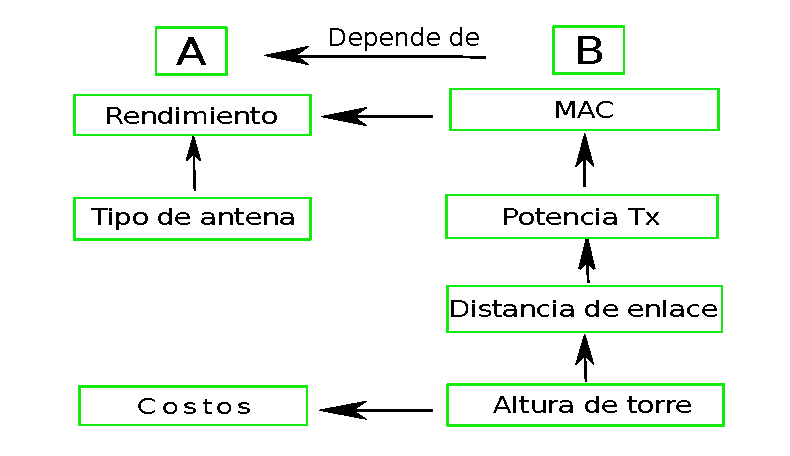
\includegraphics[width=0.70000\textwidth]{dependencias.pdf}
\caption{Dependencias de requermientos a demás}
\end{figure}

Basado en un proyecto titulado ´Digital Gangetic Plains´ los autores
argumentan que el costo principal en redes de larga distancia con 802.11
es el conjunto de torres de antenas, puesto que una antena puede valer
\$50, una torre de 30 m puede valer \$1000, por esto es de vital
importancia tener una buena planeación en la primera decisión de
despliegue; la tesis de \emph{Sayandeep Sen y Bhaskaran Raman} {[}{]} se
enfoca en que el principal problema es minimizar los costos, por esto se
hace énfasis en la planeación de una topología de red inalámbrica
optimizando los costos el despliegue, cabe destacer que al igual que
\emph{Bernardi} el despliegue con redes Ad-hoc no presta atención al
costo del sistema y no permite escalar a grandes redes. Como
característica definida se tiene que la falta de planificación impide
que se garantice el rendimiento de la red.

Para la formulación en la construcción de una topología que permita el
rendimiento de la red, se estipulan de tres principales restricciones:

\begin{enumerate}
\def\labelenumi{\arabic{enumi}.}
\tightlist
\item
  Aplicación (restricción de rendimiento): Capacidad de carga y descarga
  por cada nodo o pueblo.
\item
  Restricción de Potencia: Se refiere al límite superior de la Potencia
  Isotrópica Irradiado (PIRE) en cada transmisor y el límite inferior de
  potencia recibida en el receptor (sensibilidad del receptor).
\item
  Restricción de interferencia: La señal recibida debe ser mayor al
  umbral de interferencia.
\end{enumerate}

Los ítems 1 y 3 Usan el protocolo de control de Acceso al medio MAC, sin
embargo, {[}sent{]} plantea la implementación del protocolo 2PMAC debido
a que permite a multiples enlaces operar simultáneamente (funcionamiento
síncrono) y está específicamente diseñado para redes inalámbricas de
larga distancia. Los protocolos MAC tienen limitaciones ya sea de acceso
múltiple por división de tiempo (TDMA) o detección de portadora de
Acceso Múltiple con prevención de colisiones (CSMA/CA), una en la que
los enlaces operan en turnos predeterminados y la siguiente en la que
los enlaces no tienen un orden predeterminado compitiendo por una
pequeña duración para seleccionar el enlace que operara al mimo tiempo,
respectivamente. De acuerdo al protocolo MAC utilizado se determina el
máximo rendimiento alcanzable por un nodo en la topología y la potencia
de transmisión de cada uno de ellos.

El problema de construcción de la topología se puede establecer como:

`` \emph{Teniendo en cuenta, (a) las ubicaciones (coordenadas
\(<x, y, z>\)) de un conjunto de aldeas que se proporcionarán con
conectividad de red y la de la línea terrestre que proporciona y (b) el
requisito de ancho de banda específico por nodo de aldea, lo que es la
topología de costo mínimo que satisface las tres restricciones:
rendimiento, interferencia y potencia.} ''

\subsubsection{Consideraciones de diseño y enfoque de solución para las
variables}\label{consideraciones-de-diseuxf1o-y-enfoque-de-soluciuxf3n-para-las-variables}

\paragraph{Topología de Búsqueda
(TS):}\label{topologuxeda-de-buxfasqueda-ts}

Explorar el espacio de búsqueda para encontrar la topología de la red,
se hace uso del algoritmo Branch-and-bound (Algoritmo de ramificación y
límite), con ello se construye la topología de árbol.

\paragraph{Asignación de altura (HA):}\label{asignaciuxf3n-de-altura-ha}

Consiste en la altura óptima de las torres en las ubicaciones dadas una
vez que se ha formado la topología, para ello se utiliza un conjunto de
ecuaciones de programación lineal (LP).

\paragraph{Asignación de Antena (AA):}\label{asignaciuxf3n-de-antena-aa}

Asignación apropiada de las antenas y sus respectivas orientaciones, se
desarrolla un algoritmo heurístico de tiempo complejo polinómico.

\paragraph{Asignación de Potencias
(PA):}\label{asignaciuxf3n-de-potencias-pa}

Proporcionar las potencias de transmisión en los radios del sistema
usando LP.

El objetivo principal es el de reducir el mínimo costo de
implementación, sabiendo que el rendimiento de la red depende del tipo
de enrutamiento y del protocolo MAC implementado. Por su simplicidad se
propone la topología de árbol ya que proporciona una fácil conectividad
y para este caso no aborda la tolerancia a fallos, cabe resaltar que
utiliza un enrutamiento fijo.

El problema radica en el hecho de que las zonas rurales tienen baja
densidad de usuarios y grandes distancias entre grupos de usuarios, esto
conlleva a que compañías de telecomunicaciones o proveedores de internet
(ISP) vean poco atractiva la inversión en estos lugares debido al costo
inicial de infraestructura y despliegue de la red y bajo retorno de su
inversión.

Según Bernardi, en las últimas décadas se ha incrementado la
conectividad de banda ancha, siendo la ADSL (del inglés Asymmetric
digital subscriber line) con más del 60\% de las conexiones de banda
ancha en países de la Organización para la Cooperación y el Desarrollo
Económicos es un organismo de cooperación internacional (OCDE); esto se
debe principalmente al éxito de la capitalización de ADSL debido al
éxito de la red de telefonía. Esta tecnología se caracteriza por que la
tasa de trasmisión máxima que puede alcanzar esta en función de la
distancia entre el usuario y la central telefónica, es decir, entre más
larga sea la distancia, la velocidad de trasmisión es más lenta, por
esta razón es comúnmente más utilizada en áreas metropolitanas debido a
que tiene más suscriptores y sea más efectivo retornar la inversión de
despliegue de una infraestructura. Esto es la principal causa de la
brecha digital que existe entre las áreas rurales y metropolitanas.

El internet satelital se podría decir que es una alternativa de
conexión, puesto que está disponible prácticamente en cualquier parte y
es frecuentemente subsidiada en áreas remotas incomunicadas, sin
embargo, también tiene latencia de tiempo de ida y vuelta muy altos, lo
cual lo hace inadecuado para aplicaciones que consuman un ancho de banda
considerable, como es el caso de una videollamada (skape).

Pero Bernardi expone el Despliegue de una red Rural de Banda Ancha (BWA)
argumentando que la planeación ad-hoc no es una alternativa de diseño
eficiente para este tipo de redes, sin embargo, refiere que la industria
ofrece software para planeamiento de redes inalámbricas pero estos no
están disponibles ni son adecuados para comunicar pequeñas comunidades y
pequeños proveedores de servicio de Internet inalámbrico (WISP) ; cabe
resaltar que las BWA usan un modelo de dos niveles, consistiendo en
radioenlace Punto Multipunto (PMP) y Punto a Punto (PTP), el primero
enlazando la Antena de la torre a los diferentes clientes y el segundo
correspondiente al Backhaul. A través del planeamiento de red
incremental Bernardi desarrolla un software denominado IncrEase cuyo
enfoque es identificar la estrategia de despliegue más económica para
planear la red teniendo en cuenta que los CPE (customer Premises
Equipment) son la opción más rentable para llegar a la población en
zonas rurales.

Los proveedores de servicio de internet inalámbrico implementan una
metodología de diseño para operar en escenarios rurales obteniendo
remuneración de su inversión, este consiste en planificar su crecimiento
ampliando su cobertura, tomando variables como:

\begin{itemize}
\item
  Limitar el alcance geográfico de los WISP:Para reducir los costos de
  operación
\item
  Infraestructura de la red: En áreas rurales la fibra para el Backhaul
  no está disponible, por ello los WISP deben desplegar su propio
  Backhaul inalámbrico, aumentando los costos.
\item
  Cobertura de la red: El despliegue rural está basado en la cobertura
  más no en la capacidad
\item
  Presupuesto ajustado: Los proveedores de internet buscan obtener un
  retorno de su inversión desde su etapa de despliegue ya que las zonas
  rurales son entornos de baja rentabilidad
\item
  Clientes agrupados: Proporcionar acceso a la red en sectores dónde
  haya más densidad de la población, para así captar más usuarios.
\end{itemize}

La falta de herramientas de software para el diseño, gestión y
evaluación de redes de acceso inalámbrico de banda han obstaculizado su
despliegue generalizado a pesar de sus costos y ventajas operativas
sobre otras alternativas de Tecnologías de acceso de banda. Bernardi
desarrolla un paquete de software para llenar esta brecha, con especial
énfasis en las regiones rurales y en desarrollo. Se resalta que abordó
tres desafíos técnicos en el contexto de redes de acceso inalámbrico de
banda ancha:

\begin{itemize}
\tightlist
\item
  Mapeo de Banda Ancha
\item
  Planeación de redes
\item
  Administración de redes
\end{itemize}

\subsection{Herramienta IncrEase}\label{herramienta-increase}

Se desarrolla un software de código abierto IncrEase implementado como
una aplicación de escritorio multiplataforma en Java. IncrEase esta
basado en un GIS de software libre de la NASA World Wind Java y en una
base de datos gráfica Neo4J.

Para la implementación de IncrEase se toman tres fuentes:

\begin{itemize}
\tightlist
\item
  Demanda de la cobertura: Posibles usuarios de zonas rurales que no
  tienen acceso al servicio
\item
  Usuarios que fallaron en la etapa de instalación: Cobertura
  insuficiente
\item
  Reporte mesas de ayuda: Localización de los usuarios existentes
\end{itemize}

Además se obtienen otros datos de factores influyentes como la
disponibilidad DSL, la cobertura de red 3G y datos demográficos.
IncrEase a través de datos en forma de arreglo bidimensional cubre
regiones de interés y con ello obtiene mapas de calor (áreas de mayor
beneficio por la actualización de la red). En estos mapas a mayor calor
menor es la cobertura, una posible solución es la instalación de una
torre a partir de una lista de torres disponibles en esa área.

\subsubsection{Modo de operación herramienta
IncrEase}\label{modo-de-operaciuxf3n-herramienta-increase}

Flujo de información de la herramienta

\begin{itemize}
\item
  IncrEase Targeted: En este modo de operación el operador selecciona
  una región específica de cobertura, como parte de expansión de la red
\item
  Búsqueda Estratégica: Dónde la herramienta guía al operador para
  decidir el orden de despliegue de sitios de transmisión en el
  horizonte de corto o largo plazo basado en la rentabilidad esperada
\end{itemize}

La contribución de Bernardi es potenciar el negocio de los pequeños
proveedores de internet inalámbrico (WISP) en zonas rurales a través de
un sistema de software, haciéndolo más eficiente reduciendo la brecha
digital.

A nivel local, {[}Rios{]} propone una solución de construcción de
topología en redes rurales inalámbricas en la región del
sumapaz-Colombia. Dentro de este contexto y al igual que sen, bernardi,
maserati, expone que el principal desafío es el costo que conlleva
establecer redes en zonas rurales, haciendo especial enfásis en el costo
de construcción de las torres que soportan las antenas, debido a que es
el costo más grande en comparación con los atribuidos a los equipos de
comunicación. Presenta los siguientes referentes:

\subsubsection{Construcción de redes}\label{construcciuxf3n-de-redes}

Dentro de este campo determina elementos tales como:

\begin{itemize}
\tightlist
\item
  Costos de las torres
\item
  Baja densidad de la población
\item
  Bajo poder económico
\item
  Costos de infraestructura y equipos
\end{itemize}

\subsubsection{Topología}\label{topologuxeda}

Establece que las redes rurales mantienen una topología fija y se
realizan enlaces de larga distancia, sin embargo, al ser áreas
campestres existe una mayor cantidad de obstrucciones y acorde la
topografía varia la altura de los obstáculos.

\subsubsection{Costo de las torres}\label{costo-de-las-torres}

Para lograr obtener linea de vista entre los diferentes nodos es
necesario que las torres tengan una altura suficiente para superar los
obstáculos oresentados en el terreno. Para la construcción de estas
torres establece dos tipos de materiales:

\begin{itemize}
\tightlist
\item
  Mástiles
\item
  Torres de acero ventadas
\end{itemize}

De lo anterior determina que el coste de la torres es directamente
proporcional a su altura.

\end{document}
